\subsection{介绍TensorFlow Lite}
TensorFlow Lite是针对移动设备和嵌入式设备的TensorFlow的轻量级的解决方案。他以很低的代价和小的二进制文件尺寸在设备上进行机器学习推理。TensorFlow Lite也支持用\href{https://developer.android.com/ndk/guides/neuralnetworks/index.html?hl=zh-cn}{Android Neural Networks API}进行加速。

TensorFlow Lite用一些想优化移动app核心,预先融合激活,量化内核的技术获取更低的消耗获得更小更快的模型。
大多数的TensorFlow Lite文档在\href{https://github.com/tensorflow/tensorflow/tree/master/tensorflow/contrib/lite}{Github}上。
\subsection{TensorFlow Lite包含什么?}
TensorFlow Lite包含一系列核心操作,包括针对移动平台调整的量化和浮点。他么通过预先融合激活和偏置加强性能和量化精度。另外,TensorFlow Lite也支持在模型中使用自定义的操作。

TensorFlow Lite定义了一个新的基于\href{https://google.github.io/flatbuffers/}{FlatBuffers}模型文件格式。FlatBuffers是一个开源,高效,跨平台的序列化库。类似\href{https://developers.google.com/protocol-buffers/?hl=en}{Protocol buffers},但是主要的不同是在访问数据时FlatBuffers不需要解析/解包步骤为一个二次表达,经常和对象内存分配成对出现。FlatBuffers代码足迹比protocal buffers更小。

TensorFlow Lite是一个新的移动量化平台目标是跟中app的负载和速度。解释器用一个静态图和一个自定义的(少量动态)内存分配器企鹅报最小的砸入,初始化,和高效执行。

TensorFlow Lite 提供一个接口用于硬件加速,如果硬件加速在设备上可用。它通过Android Neural Network库(Android O-MR1)加速。
\subsection{为什么需要一个新的专为移动平台设计的库?}
机器学习正在改变计算范式,我们看到了嵌入式平台和移动平台融合的趋势。用户期望和他们的设备通过摄像头,声音交互模型以自然,人类喜欢的方式交互。
下面是融合的一些因素:
\begin{itemize}
\item 在半导体硅上的创新是硬件加速的新的可能,想Android Neural Network API框架使得利用硬件加速成为可能
\item 现在先进的实时计算机视觉和语义理解一定导致移动优化基准模型正在被开源
\item 在设备智能上为广泛的智能应用创建了新的可能。
\item 对用户数据隐私不需要离开移动设备的兴趣
\item 服务离线情况,这里的设备不需要连接网络
\end{itemize}
我们相信下一波机器学习应用浪潮将来自于移动平台和嵌入式设备。
\subsection{TensorFlow Lite 开发者预览重点}
作为开发者预览的TensorFlow Lite包含如下内容:
\begin{itemize}
\item 包括量化的和浮点的核心操作已经被转化用于移动平台。这可能用于创建和运行自定义的模型。开发者可以在他们的模型中写自己的操作
\item 一个新的\href{https://google.github.io/flatbuffers/}{FlatBuffers}模型文件格式
\item 结合内和核心优化在移动设备上更快的执行
\item TensorFlow转化器转化TensorFlow-trained的模型为TensorFlow Lite格式
\item 更小的尺寸:TensorFlow Lite当所有的操作被连接小于300KB,当用操作徐娅支持Inception V3和MobileNet时小于200KB
\item 预先测试的模型:所有的模型被确保效果\begin{itemize}
\item Inception V3,一个流行在图像上的侦测对象的模型
\item \href{https://github.com/tensorflow/models/blob/master/research/slim/nets/mobilenet_v1.md}{MobileNets}当用于资源受限的设备或者谦如水应用的一个熟悉的针对移动平台的高效的最大化精确度计算机视觉模型。塔恩很小,低时延,低功耗模型参数化以范主各种资源受限的情况。他们能被构建用于分类,检测,嵌入和分割。MobileNet模型很小但是相比Inception V3\href{https://research.googleblog.com/2017/06/mobilenets-open-source-models-for.html}{精度低}
\item 在设备智能回复,在设备模型上对输入文本信息给出相关的建议信息回复。模型被构建用于内存有限的设备像手表和手机等设备上并且他对于第一方和第三方app已经被成功的用于\href{https://research.googleblog.com/2017/02/on-device-machine-intelligence.html}{Smart Replies onAndroid Wear}
\item 量化的MobileNet模型版本,运行比没有量化的版本在CPU上运行更快
\item 新的Android示例程序解释TensorFlow Lite结合量化的MobileNet模型用于目标检测是如何使用的
\item Java 和C++ API支持
\end{itemize}
\end{itemize}
\begin{quote}
这是一个开发者版本,可能子啊将来的API中修改,我们不能保证这个版本向后兼容
\end{quote}
\subsection{开始}
我们推荐你结合上面的预先测试好的模型进行尝试。如果你有一个存在的模型,你讲需要测试是否你的模型和转化器和支持的操作集合兼容。为了测试模型,查看\href{https://github.com/tensorflow/tensorflow/tree/master/tensorflow/contrib/lite}{documenttation on GitHub}
\subsection{重新训练Inception V3或者MobileNet用于用户自定义的数据集}
上面提到的模型是基于ImageNet数据集1000个分类的数据进行训练的。如果这些类对你的使用不相关或者没用,你将需要重新训练模型。这个技术成为迁移学习,在一个已经训练好的模型上重新训练一个类似的问题。深度学习训练可能花费很长时间,但是迁移学习能以被很快的使用。为了做这个事,你将需要生成你的自定义的数据集结合相关的类标记。

\href{https://codelabs.developers.google.com/codelabs/tensorflow-for-poets/?hl=zh-cn}{TensorFlow for Poets}代码实验室告诉你如何一步步左到。重新训练代码支持重新训练用于浮点和量化接口。
\subsection{TensorFlow Lite 架构}
下面的图显示了TensorFlow Lite的架构设计
\begin{figure}[H]
\centering
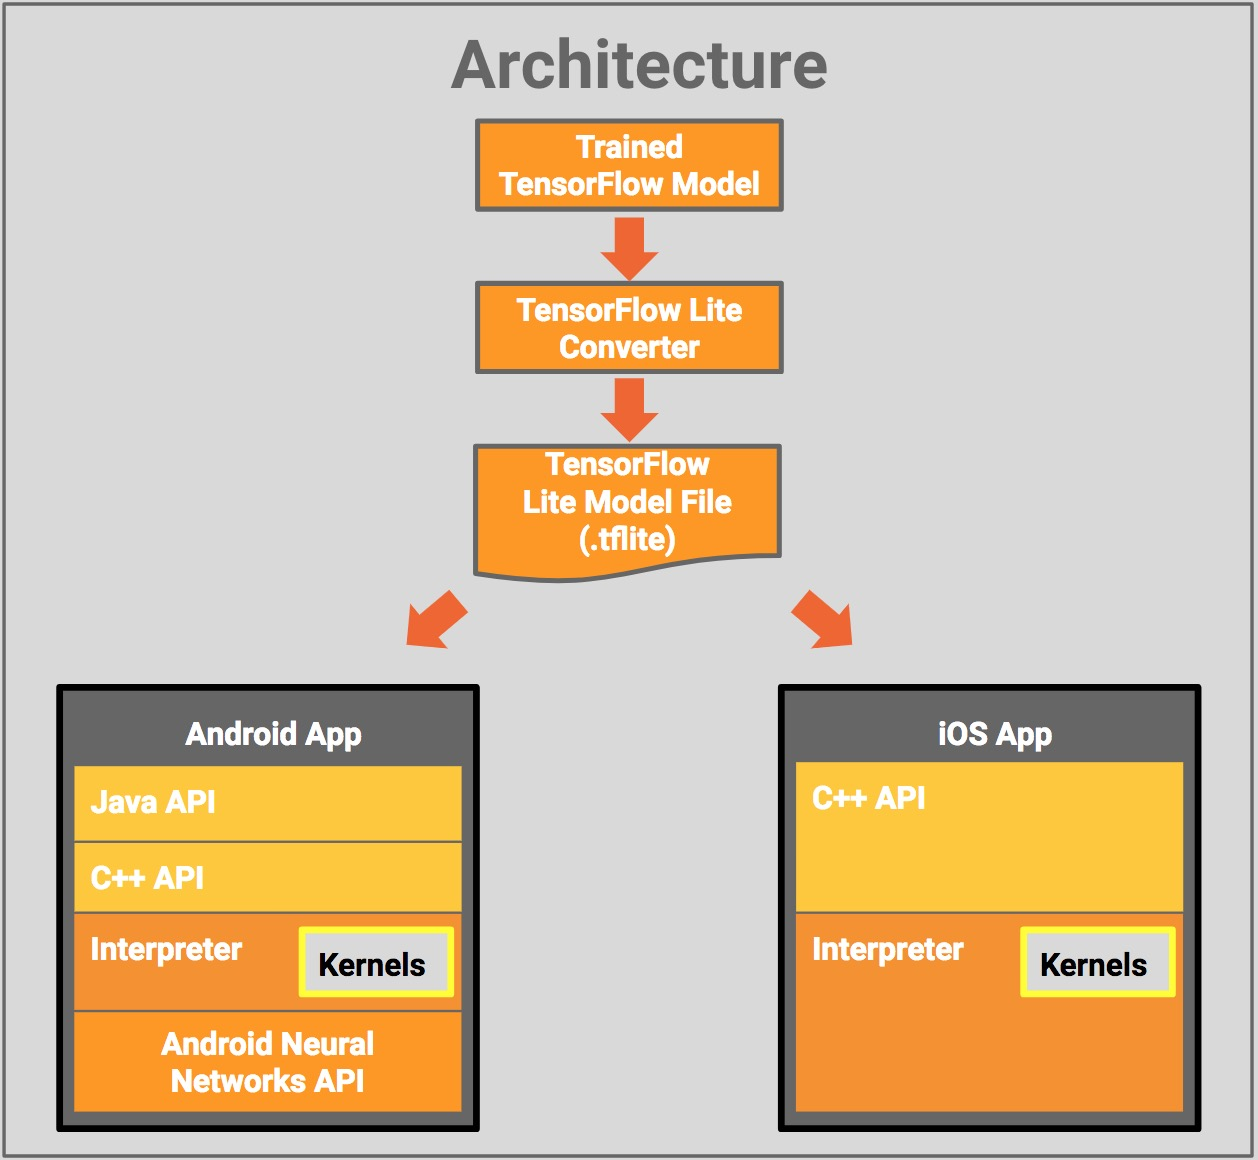
\includegraphics[scale=0.3]{tflite-architecture.jpg}
\caption{TensorFlow Lite 架构}
\end{figure}
在磁盘上开始一个训练的模型,你将用TensorFlow Lite转化器转化模型为TensorFlow Lite文件格式(.tflite)。然后你可以用转化的文件在你的移动应用上。
部署TensorFlow Lite模型文件:
\begin{itemize}
\item Java API:一个方便的在Android上围绕C++ API的包装器
\item C++ API:载入TEnsorFlow Lite模型文件,调用解释器,相同的库在Android和IOS上都可用
\item 解释器:用一些可信执行模型。解释器支持选择核心载入;没有核心仅仅100KB,3,全部载入核心300KB。这是从TensorFlow Mobile要求的1.5M重要的减小
\item 在选择的Android设备上,解释器讲用Android Neural Network API用于硬件加速,或者如果没有可用的默认使用CPU执行。
\end{itemize}
你可以用C++ API实现用于解释器的自定义核心。
\subsection{将来的工作}
在将来的版本中TensorFlow Lite讲支持更多的模型和内建操作,包括用于对固定点和浮点模型的运行改进,和让开发者更容易的开发工作刘和对其它更小的设备的支持等等。正如我们继续开发,我们希望TensorFlow Lite将简化开发者对于小型设备的开发者经历。

将来几哈用指定的机器学习硬件获取更好的可能性能用于类似设备上的类似模型。
\subsection{下一步}
对于开发者预览,多数文档在GitHub上。请查看\href{https://github.com/tensorflow/tensorflow/tree/master/tensorflow/contrib/lite}{TensorFlow Lite repository}获取更多信息和代码样例,事例应用和更多。

